\section{Orientation of a regular surface}
\begin{question}
    Consider \(\mathbb{S}^2\) with spherical parametrization, are following two
    parametrizations the same?
    \begin{itemize}
        \item \((\vphi,\theta)\longmapsto(\sin\vphi\cos\theta,\sin\vphi\sin\theta,
            \cos\vphi)\)
        \item \((\theta,\vphi)\longmapsto(\sin\vphi\cos\theta,\sin\vphi\sin\theta,
            \cos\vphi)\)
    \end{itemize}
\end{question}

The answer is NO\@! They give different normal directions which decide ``inside'' and
``outside'' of \(\mathbb{S}^2\).

\noindent\underline{\bfseries Recall:} \(\mathbb{R}^2\) is orientable. It has two
orientations. Given a basis \(\{e_1,e_2\}\), let
\begin{align*}
    J_{+}=\Bigl\{E_{+}=\{e_1^+,e_2^+\}&:E_{+}\text{ has same orientation as }E.\\
    &\text{ \ie\ }\begin{bmatrix}
        e_1^+\\ e_2^+
    \end{bmatrix}=\underbrace{\begin{bmatrix}
        a_{11} & a_{12} \\
        a_{21} & a_{22}
    \end{bmatrix}}_{A_{+}}\begin{bmatrix}
        e_1 \\ e_2
    \end{bmatrix}
    \text{ and }\det A_{+}>0\Bigr\};
\end{align*}
\begin{align*}
    J_{-}=\Bigl\{E_{-}=\{e_1^-,e_2^-\}&:E_{-}\text{ has same orientation as }E.\\
    &\text{ \ie\ }\begin{bmatrix}
        e_1^-\\ e_2^-
    \end{bmatrix}
    =A_{-}\begin{bmatrix}
        e_1 \\ e_2
    \end{bmatrix}
    \text{ and }\det A_{-}>0\Bigr\}.
\end{align*}
Then either \(J_{+}\) or \(J_{-}\) gives an orientation of \(\mathbb{R}^2\).

\begin{question}\hfill
\begin{enumerate}[(1)]
    \item Let \(S\) be a regular surface, how can we define orientation?
    \item Are all surfaces orientable?
\end{enumerate}
\end{question}

Assume we have two parametrizations around \(p\):
\begin{align*}
    F&\colon U\to S &&T_p S\cong \mathbb{R}^2=\Span\{F_u,F_v\} \\
    G&\colon V\to S &&T_p S\cong \mathbb{R}^2=\Span\{G_\alpha,G_\beta\}
.\end{align*}
Note near \(p\), \(F(u,v)=G(\alpha,\beta)\implies \) \[
    \begin{bmatrix}
        G_\alpha \\ G_\beta
    \end{bmatrix}=\begin{bmatrix}
        u_\alpha & v_\alpha \\
        u_\beta & v_\beta
    \end{bmatrix}\begin{bmatrix}
        F_u \\ F_v
    \end{bmatrix}
.\] 
\ie\ Two parametrizations \(F\) and \(G\) give the same orientation iff \[
    \left|\pdv{(u,v)}{(\alpha,\beta)}\right|>0
.\] 

\begin{definition}[Orientation of a regular surface]
    We say a regular surface \(S\) is orientable if there exists a coordinate
    chart covering of \(S\), \st\ if a point \(p\) belongs to two charts, then the
    induced basis on \(T_p S\) by the two parametrizations have the same orientation
    in above sense.
\end{definition}

\begin{remark}\hfill
\begin{enumerate}[(1)]
    \item ``Orientation'' is a global intrinsic property. ``Orientability'' is
    essentially reflected by the topology of the surface. In algebraic topology
    course, you'll see that the orientability is determined by the 1st
    Stiefel-Whitney class in \(H^1(M,\mathbb{Z}/2\mathbb{Z})\) for a vector
    bundle on topological manifold \(M\).
    With additional ``smooth'' structure on \(M\), we have more ways to check
    the orientability, for example, \(\exists\) a nowhere vanishing top
    differential form (or say, a volume form).
    \item One of important applications of ``orientation'' in this course (and
    later in Reimann Geometry) is allowing us to define ``integration'' on a regular
    surface.
\end{enumerate}
\end{remark}

\begin{exercise}
    Give a definition of orientation of \(\mathbb{R}^n\) as a vector space.
\end{exercise}

\begin{example}
    \(\mathbb{S}^2\) is orientable.
\end{example}

Consider the stereographic parametrization
\begin{align*}
    \pi_N\colon \mathbb{S}^2\setminus\{N\} &\longrightarrow \mathbb{R}^2 \\
    (x,y,z) &\longmapsto (u,v)=(\frac{x}{1-z},\frac{y}{1-z})
.\end{align*} \[
    \pi_N^{-1}(u,v)=(\frac{2u}{1+u^2+v^2},\frac{2v}{1+u^2+v^2},1-\frac{2}{1+u^2+v^2})
.\] \begin{align*}
    \pi_S\colon \mathbb{S}^2\setminus\{S\} &\longrightarrow \mathbb{R}^2 \\
    (x,y,z) &\longmapsto (\alpha,\beta)=(\frac{y}{1+z},\frac{x}{1+z})
.\end{align*} \[
    \pi_N^{-1}(\alpha,\beta)=(\frac{2\beta}{1+\alpha^2+\beta^2},\frac{2\alpha}
    {1+\alpha^2+\beta^2},\frac{2}{1+\alpha^2+\beta^2}-1)
.\] Clearly \(\mathbb{S}^2=\pi_N^{-1}(U)\cup \pi_S^{-1}(V)\). To see the orientation,
we compute the Jacobian of change form one chart to another. \((u,v)\to (\alpha,\beta
)\). Now \[
    \begin{cases}
        u=\frac{x}{1-z} \\
        v=\frac{y}{1-z}
    \end{cases},\quad
    \begin{cases}
        \alpha=\frac{y}{1+z} \\
        \beta=\frac{x}{1+z}
    \end{cases}
.\] Hence \[
    \begin{cases}
        u\alpha=v\beta \\
        u\beta+v\alpha=1
    \end{cases}\implies \ \ 
    \begin{cases}
        u=\frac{\beta}{\alpha^2+\beta^2} \\
        v=\frac{\alpha}{\alpha^2+\beta^2}
    \end{cases}
.\] Then \[
    \pdv{(u,v)}{(\alpha,\beta)}=\begin{pmatrix}
        -\frac{2\alpha\beta}{(\alpha^2+\beta^2)^2} &
        \frac{\alpha^2-\beta^2}{(\alpha^2+\beta^2)^2} \\
        \frac{\beta^2-\alpha^2}{(\alpha^2+\beta^2)^2} &
        -\frac{2\alpha\beta}{(\alpha^2+\beta^2)^2}
    \end{pmatrix}\implies \det>0
.\] 

\begin{example}
    The graph \((x,y,f(x,y))\) is always orientable.
\end{example}

\noindent\textbullet{} Normal vector field and orientation.

Since in this course, we consider the regular surface \(S\) in \(\mathbb{R}^3\),
at each \(p\in S\), there is a unique tangent plane \(T_p S\), which is a 2 dim
linear subspace of \(\mathbb{R}^3\). Hence we can talk abort the normal vector
field on \(S\). Now we want a ``well-defined'' normal by taking ``unit normal vector
\(\vec{n}\)'' at \(p\).

Let's check \(\vec{n}\) under change of parameter. Let \(F\colon U\to S\) be
a parametrization around \(p\). Then \[
    T_p S=\Span\{F_u,F_v\}\implies\vec{n}_F=\frac{F_u\times F_v}{|F_u\times F_v|}
.\] (Note the cross product here already assigns a direction of \(\vec{n}\)).

If \(G\colon V\to S\) is another parametrization around \(p\). Then \[
    T_p S=\Span\{G_\alpha,G_\beta\},\quad \vec{n}_G=\frac{G_\alpha\times G_\beta}
    {|G_\alpha\times G_\beta|}
.\] Let \(\Phi=G^{-1}\circ F\colon U\cap V\to U\cap V\) be the transition map.
Then \[
    \begin{cases}
        F_u=G_\alpha\alpha_u+G_\beta\beta_u \\
        F_v=G_\alpha\alpha_v+G_\beta\beta_v
    \end{cases}
    \text{\ie\ }
    \begin{pmatrix}
        F_u \\ F_v
    \end{pmatrix}=\begin{pmatrix}
        \alpha_u & \beta_u \\
        \alpha_v & \beta_v
    \end{pmatrix}\begin{pmatrix}
        G_\alpha \\ G_\beta
    \end{pmatrix}
.\]
\(\implies F_u\times F_v=\det(\pdv{(\alpha,\beta)}{(u,v)})G_\alpha\times G_\beta\).
Hence \[
    \vec{n}_F=\sign \det(\pdv{(\alpha,\beta)}{(u,v)})\cdot \vec{n}_G
.\] 

\begin{definition}[Unit normal vector field]
    \(U\subset S\) open subset, a unit normal vector field on \(U\) is a smooth map
    \begin{align*}
        \vec{n}\colon U &\longrightarrow \mathbb{R}^3 \\
        p &\longmapsto \vec{n}_p\text{ (unit normal at }p\text{)}
    .\end{align*}
\end{definition}

\begin{prop}
    A regular surface is orientable \(\iff \) there is a unit normal vector field
    \(\vec{n}\colon S\to \mathbb{R}^3\) defined everywhere on \(S\).
\end{prop}

\begin{remark}
    On an orientable regular surface, the ``unit'' normal vector field has image
    on \(\mathbb{S}^2\), \ie\ there is a smooth map 
    \begin{align*}
        \vec{n}\colon S &\longrightarrow \mathbb{S}^2=\{x^2+y^2+z^2=1\} \\
        p &\longmapsto \vec{n}_p
    .\end{align*}
    This \(\vec{n}\) is called the \emph{Gauss map} of the surface. Later we'll
    see that the differential of \(\vec{n}\) determines how the surface is curved
    in \(\mathbb{R}^3\).
\end{remark}

\begin{proof}
    ``\(\implies \)'': If \(S\) is orientable, then \(\exists\) a coordinate chart
    covering \(\{F_\alpha(U_\alpha)\}_{\alpha\in \Lambda}\) of \(S\),
    (\(F_\alpha\colon U_\alpha\to S,S=\bigcup_{\alpha\in \Lambda}F_\alpha(U_\alpha)
    \)). \st\ on \(U_\alpha\cap U_\beta\neq \emptyset\), \[
        \det(\pdv{(u_\alpha,u_\beta)}{(u_\beta,v_\beta)})>0
    .\] Hence at \(p\in U_\alpha\cap U_\beta\), \[
        \vec{n}_p
        =\frac{F_{u_\alpha}\times F_{v_\alpha}}{|F_{u_\alpha}\times F_{v_\alpha}|}
        =\frac{F_{u_\beta}\times F_{v_\beta}}{|F_{u_\beta}\times F_{v_\beta}|}
    .\] (This guarantees that we can extend the normal vector in on chart to another)
    
    Hence we can well define \(\vec{n}\colon S\to \mathbb{R}^3\). The smoothness of
    \(\vec{n}\) can be checked in local coordinates.

    ``\(\impliedby \)'': Let \(\vec{n}\colon S\to \mathbb{R}^3\) be the unit normal
    vector field defined on \(S\). Let \(\{F_\alpha\colon U_\alpha\to S\}\) be a
    coordinate chart covering of \(S\). Then on each \(F_\alpha(U_\alpha)\), \[
        \vec{n}_\alpha
        =\frac{F_{u_\alpha}\times F_{v_\alpha}}{|F_{u_\alpha}\times F_{v_\alpha}|}
    .\] On \(U_\alpha\cap U_\beta\) at some point \(p\), we have \[
        \frac{F_{u_\alpha}\times F_{v_\alpha}}{|F_{u_\alpha}\times F_{v_\alpha}|}
        =\sign \det(\pdv{(u_\beta,v_\beta)}{(u_\alpha,v_\alpha)})\cdot 
        \frac{F_{u_\beta}\times F_{v_\beta}}{|F_{u_\beta}\times F_{v_\beta}|}
    .\] Since \(\vec{n}_\alpha\) and \(\vec{n}_\beta\) agree at \(p\), we see \[
        \det(\pdv{(u_\beta,v_\beta)}{(u_\alpha,v_\alpha)})>0
    .\] 
\end{proof}

\begin{figure}[htb]
    \centering
    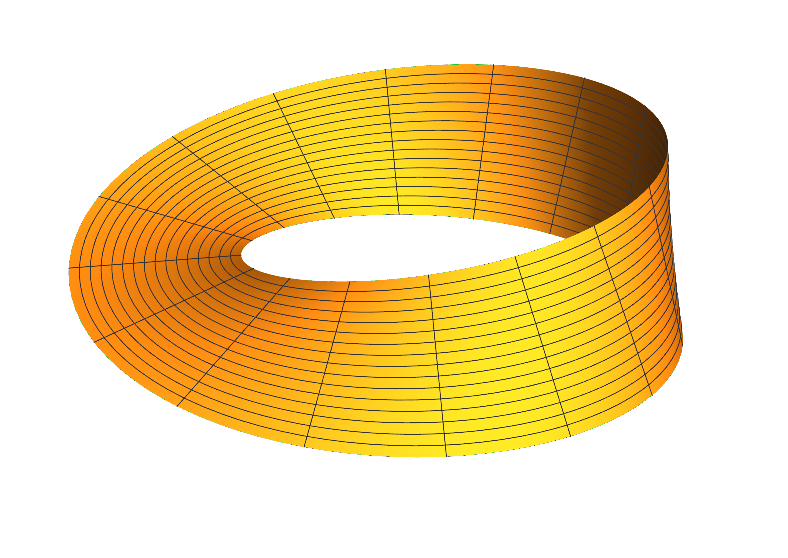
\includegraphics[width=0.5\textwidth]{picture/week6/mobius.pdf}
    \caption{M\"obius strip}\label{fig:mobius}
\end{figure}

\begin{example}[Non-orientated surface]
    M\"obius strip \(M\) (\cref{fig:mobius})
\end{example}

Consider the line segment \(AB\) with equation \(-\frac{1}{2}\le z\le \frac{1}{2},
y=1,x=0\), rotating along a circle \(x^2+y^2=1\). When the center \(c\) moves
about angle \(u\) away from \(y\)-axis, the line \(A'B'\) is in the plane determined
by \(z\)-axis and \(c'\) and the angle between \(A'B'\) and \(z\)-axis is
\(\frac{u}{2}\).

Let \(U=\{(u,v):0<u<2\pi,-\frac{1}{2}<v<\frac{1}{2}\}\), then \[
    F(u,v)=((1-v\sin\frac{u}{2})\sin u,(1-v\sin \frac{u}{2})\cos u,v\cos\frac{u}{2})
.\] This almost covers \(M\), except at \(u=0\). To cover this, we consider
rotation \(AB\) when the center lies on \(x\)-axis. We have parametrization \[
    G(\alpha,\beta)=((1-\beta\sin(\frac{\pi}{4}+\frac{\alpha}{2}))\cos\alpha,
    (1-\beta\sin(\frac{\pi}{4}+\frac{\alpha}{2}))\sin\alpha,
    \beta\cos(\frac{\pi}{4}+\frac{\alpha}{2}))
.\] \[
    V=\{(\alpha,\beta):0<\alpha<2\pi,-\frac{1}{2}<\beta<\frac{1}{2}\}
.\] Now the missing part is on \(u=\frac{\pi}{2}\).

Consider \(F(U)\cap G(V)\), it contains two pieces \[
    W_1=\{F(u,v):0<u<\frac{\pi}{2}\},\quad
    W_2=\{F(u,v):\frac{\pi}{2}<u<2\pi\}
.\] On \(W_1\), \[
    \begin{cases}
        \alpha=u+\frac{3}{2}\pi \\
        \beta=-v
    \end{cases}
    \implies \ \ \left|\pdv{(\alpha,\beta)}{(u,v)}\right|=-1
.\] On \(W_2\), \[
    \begin{cases}
        \alpha=u-\frac{\pi}{2} \\
        \beta=v
    \end{cases}
    \implies \ \ \left|\pdv{(\alpha,\beta)}{(u,v)}\right|=1
.\] No matter how we change parametrization in \(W_1\) or \(W_2\), we can not
guarantee that \(\left|\pdv{(\alpha,\beta)}{(u,v)}\right|\) is positive everywhere.
(\ie\ \(\vec{n}\) has to change sign). Hence \(M\) is non-orientable.

\begin{remark}
    In the following of this course, we only care about orientable surfaces.
    \ie\ surfaces having well-defined unit normal vector field everywhere.
\end{remark}

\section{The \texorpdfstring{\engordnumber{1}}{1st} fundamental form on \texorpdfstring{\(S\)}{S}}

The \engordnumber{1} fundamental form on \(S\) inherits from the Euclidean inner product of
\(\mathbb{R}^3\). It allows us to measure geometric quantities like
\begin{itemize}
    \item Distance between pairs;
    \item Angle between curves;
    \item Area of a region;
    \item etc.
\end{itemize}
It is an intrinsic, globally defined concept on \(S\). In the language of Riemannian
Geometry, the 1st fundamental form is also called the ``pull-back'' Riemannian
metric on \(S\). It's related to the ``isometric immersion (embedding)'' in 
Riemannian Geometry course.

\begin{center}
\textcolor{red}{
    \textbf{\large!} The 1st fundamental form determines the ``intrinsic
    geometry''.
}
\end{center}

We first give the definition of the 1st fundamental form, then explain where it
comes from.

Let \(S\subset \mathbb{R}^3\) be a regular surface. \(\forall\,p\in S\), we take
local parametrization
\begin{align*}
    \vphi\colon U\subset \mathbb{R}^2 &\longrightarrow S \\
    (u,v)&\longmapsto \vphi(u,v)=(x,y,z)
.\end{align*}
and \(p=\vphi(u_0,v_0)\), then 
\begin{align*}
    \vphi_u(u_0,v_0)&=\eval{(x_u,y_u,z_u)}_{(u_0,v_0)}\in \mathbb{R}^3 \\
    \vphi_v(v_0,v_0)&=\eval{(x_v,y_v,z_v)}_{(u_0,v_0)}\in \mathbb{R}^3
.\end{align*}
And \(T_p S\cong \mathbb{R}^2=\Span\{\vphi_u(u_0,v_0),\vphi_v(u_0,v_0)\}\).

Define \[
    E=\left<\vphi_u,\vphi_u\right>_p\quad F=\left<\vphi_u,\vphi_v\right>_p\quad
    G=\left<\vphi_v,\vphi_v\right>.
\] The 1st fundamental form at \(p\in S\) is defined as \[
    I_p=E\dd{u}^2+2F\dd{u}\dd{v}+G\dd{v}^2
.\] To understand this, let's start with inner product in \(\mathbb{R}^3\). \[
    \mathbb{R}^3=\Span\{e_1,e_2,e_3\}=\Span\{\pdv{x},\pdv{y},\pdv{z}\}
    =\Span\{\pdv{x^1},\pdv{x^2},\pdv{x^3}\}.
\] Here, since for each vector \(v\) with length 1, it uniquely determines a
directional derivative \(\nabla_v\) and vice versa.
Hence we can identify \(e_1=(1,0,0)\) with \(\pdv{x^1}\), and \(e_2=\pdv{x^2}\),
\(e_3=\pdv{x^3}\).

The inner product on \(\mathbb{R}^3\) is
\begin{align*}
    g_{\mathbb{R}^3}\colon\mathbb{R}^3\times\mathbb{R}^3&\longrightarrow\mathbb{R}\\
    (v,w) &\longmapsto \left<v,w\right>,
    \quad v,w \text{ vectors in }\mathbb{R}^3
.\end{align*}
Satisfy:
\begin{itemize}
    \item \(g(v,w)=g(w,q)\)
    \item \(g(av_1+bv_2,w)=ag(v_1,w)+bg(v_2,w)\)
    \item \(g(v,v)\ge 0\) and \(g(v,v)=0\iff v=0\).
\end{itemize}
If \(v=\sum_{i=1}^3 v^i\pdv{x^i},w=\sum_{j=1}^{3}w^j\pdv{x^j}\), then \[
    g_{\mathbb{R}^3}(v,w)=\sum_{i,j=1}^{3}\delta_{ij}v^i w^j,
    \quad \text{where }\delta_{ij}=\begin{cases}
        1 & i=j\\
        0 & i\neq j
    \end{cases}
.\] 

\((\mathbb{R}^3)^*\), dual space of \(\mathbb{R}^3\) is defined as follows:\\
For a vector \(v\in \mathbb{R}^3\), we define an element \(\alpha_v\in(\mathbb{R}^3)
^*\) by \[
    \alpha_v=g_{\mathbb{R}^3}(v,\cdot)\colon \mathbb{R}^3\to R, \quad 
    w\mapsto \alpha_v(w)=g_{\mathbb{R}^3}(v,w)
.\] The dual basis of \(\{e_1,e_2,e_3\}=\{\pdv{x^1},\pdv{x^2},\pdv{x^3}\}\) is \[
    \{e_1^*,e_2^*,e_3^*\}=\{\dd{x^1},\dd{x^2},\dd{x^3}\}
.\] \st\ \(e_i^*(e_j)=g(e_i,e_j)=\delta_{ij}\). Then \((\mathbb{R}^3)^*=\Span
\{e_1^*,e_2^*,e_3^*\}=\Span\{\dd{x^1},\dd{x^2},\dd{x^3}\}\). Hence \[
    \alpha_v=\sum_{i=1}^3 v^i \dd{x^i},\quad
    v^1=\left<v,\pdv{x^i}\right> ,\quad
    g_{\mathbb{R}^3}(v,\cdot)=\alpha_v\in (\mathbb{R}^3)^*
.\] By relaxing \(v\) in \(g_{\mathbb{R}^3}(v,\cdot)\), we can view \(g_{\mathbb{R}
^3}\) as a symmetric element in \((\mathbb{R}^3)^*\otimes (\mathbb{R}^3)^*\).
From linear algebra, \[
    \mathrm{Sym}((\mathbb{R}^3)^*\otimes (\mathbb{R}^3)^*)=
    \Span\{\dd{x^i}\dd{x^j}=\dd{x^j}\dd{x^i}\}_{i,j=1,2,3}
.\] Hence we can write \[
    g_{\mathbb{R}^3}=\delta_{ij}\dd{x^i}\dd{x^j}=
    (\dd{x^1})^2+(\dd{x^2})^2+(\dd{x^3})^2
.\] Now let \(S\subset \mathbb{R}^3\) with local parametrization given at the
beginning of this section, \ie\ \(x^i=x^i(u,v)\). We have \[
    \dd{x^1}=x_u^1\dd{u}+x_v^1\dd{v},\quad
    \dd{x^2}=x_u^2\dd{u}+x_v^2\dd{v},\quad
    \dd{x^3}=x_u^3\dd{u}+x_v^3\dd{v}
.\] Then we consider restrict \(g_{\mathbb{R}^3}\) on \(TS\),
\begin{align*}
    g_{\mathbb{R}^3}|_{TS}
    &=(x_u^1\dd{u}+x_v^1\dd{v})^2+(x_u^2\dd{u}+x_v^2\dd{v})^2
    +(x_u^3\dd{u}+x_v^3\dd{v})^2 \\
    &=\left((x_u^1)^2+(x_u^2)^2+(x_u^3)^2\right)\dd{u}^2
    +2(x_u^1x_v^1+x_u^2+x_v^2+x_u^3x_v^3)\dd{u}\dd{v} \\
    &\quad+\left((x_v^1)^2+(x_v^2)^2+(x_v^3)^2\right)\dd{v}^2 \\
    &=\left<\vphi_u,\vphi_u\right>\dd{u}^2+2\left<\vphi_u,\vphi_v\right>\dd{u}\dd{v}
    +\left<\vphi_v,\vphi_v\right>\dd{v^2} \\
    &=E\dd{u^2}+2F\dd{u}\dd{v}+G\dd{v}^2
.\end{align*}
Therefore, we see the 1st fundamental form is just the restriction of Euclidean
inner product of \(\mathbb{R}^3\) on \(TS\).

\underline{Recall:} \(\vphi\colon U\subset \mathbb{R}^2\to S,p\in S\), then \[
    \dd{\vphi_p}\colon T_{(u_0,v_0)}U\to T_p S,
    \quad T_{(u_0,v_0)}U\cong \mathbb{R}^2=\Span\{\pdv{u},\pdv{v}\}.
\] Then \[
    \dd{\vphi_p}(\pdv{u})=\vphi_u,\quad \dd{\vphi_p}(\pdv{v})=\vphi_v
.\] We get
\begin{align*}
    I_p(\pdv{u},\pdv{u})&=E=g_{\mathbb{R}^3}(\vphi_u,\vphi_u)
    =g_{\mathbb{R}^3}(\dd{\vphi_p}(\pdv{u}),\dd{\vphi_p}(\pdv{u})) \\
    I_p(\pdv{u},\pdv{v})&=E=g_{\mathbb{R}^3}(\vphi_u,\vphi_v)
    =g_{\mathbb{R}^3}(\dd{\vphi_p}(\pdv{u}),\dd{\vphi_p}(\pdv{v})) \\
    I_p(\pdv{v},\pdv{v})&=E=g_{\mathbb{R}^3}(\vphi_v,\vphi_v)
    =g_{\mathbb{R}^3}(\dd{\vphi_p}(\pdv{v}),\dd{\vphi_p}(\pdv{v}))
.\end{align*}

Therefore, the 1st fundamental form is a positive definite bilinear form
defined on \(T_p S\cong T_{(u_0,v_0)}U\).

\begin{remark}
    In Riemannian Geometry, the generalization of above defines a ``pull-back''
    metric \(\vphi^*g\) by \(\vphi\colon M\to N\).
\end{remark}

\begin{exercise}
    Consider a vector \(v\in T_p S\), compute \(I_p(v,v)\).
\end{exercise}

\begin{remark}
    Since \(I_p=(\dd{u},\dd{v})\begin{pmatrix}
        E & F \\
        F & E
    \end{pmatrix}\begin{pmatrix}
        \dd{u} \\ \dd{v}
    \end{pmatrix}\), we might also refer \(\begin{pmatrix}
        E & F \\
        F & G
    \end{pmatrix}\) as the 1st fundamental form.
\end{remark}

\begin{theorem}
    \(I\) is independent of local parametrization.
\end{theorem}
\begin{proof}
    Let \(\vphi(u,v)\) and \(\psi(\alpha,\beta)\) be two local parametrizations
    near \(p\). \[
        \begin{cases}
            u=u(\alpha,\beta) \\
            v=v(\alpha,\beta)
        \end{cases}
        \text{ has inverse }
        \begin{cases}
            \alpha=\alpha(u,v) \\
            \beta=\beta(u,v)
        \end{cases}
    .\] Then \[
        \begin{pmatrix}
            \dd{u} \\ \dd{v}
        \end{pmatrix}=\begin{pmatrix}
        u_{\alpha} & u_\beta \\
        v_\alpha & v_\beta
        \end{pmatrix}\begin{pmatrix}
            \dd{\alpha} \\ \dd{\beta}
        \end{pmatrix}=\pdv{(u,v)}{(\alpha,\beta)}\begin{pmatrix}
            \dd{\alpha} \\ \dd{\beta}
        \end{pmatrix}
    .\] \[
        \begin{pmatrix}
            \left<\vphi_u,\vphi_v\right> & \left<\vphi_u,\vphi_v\right> \\
            \left<\vphi_v,\vphi_u\right> & \left<\vphi_v,\vphi_v\right> 
        \end{pmatrix}=\begin{pmatrix}
            \alpha_u & \beta_u \\
            \alpha_v & \beta_v
        \end{pmatrix}\begin{pmatrix}
        \left<\psi_\alpha,\psi_\beta\right> & \left<\psi_\alpha,\psi_\beta\right> \\
        \left<\psi_\beta,\psi_\alpha\right> & \left<\psi_\beta,\psi_\beta\right> 
        \end{pmatrix}\begin{pmatrix}
            \alpha_u & \alpha_v \\
            \beta_u & \beta_v
        \end{pmatrix}
    .\] This gives
    \begin{align*}
        &(\dd{u},\dd{v})
        \begin{pmatrix}
            \left<\vphi_u,\vphi_v\right> & \left<\vphi_u,\vphi_v\right> \\
            \left<\vphi_v,\vphi_u\right> & \left<\vphi_v,\vphi_v\right> 
        \end{pmatrix}\begin{pmatrix}
        \dd{u} \\ \dd{v}
        \end{pmatrix} \\
        =&(\dd{\alpha},\dd{\beta})\underbrace{\begin{pmatrix}
            u_\alpha & u_\beta \\
            v_\alpha & v_\beta
            \end{pmatrix}\begin{pmatrix}
            \alpha_u & \alpha_v \\
            \beta_u & \beta_v
        \end{pmatrix}}_{\mathrm{Id}}\begin{pmatrix}
        \left<\psi_\alpha,\psi_\beta\right> & \left<\psi_\alpha,\psi_\beta\right> \\
        \left<\psi_\beta,\psi_\alpha\right> & \left<\psi_\beta,\psi_\beta\right> 
        \end{pmatrix}\underbrace{\begin{pmatrix}
            \alpha_u & \alpha_v \\
            \beta_u & \beta_v
        \end{pmatrix}\begin{pmatrix}
            u_\alpha & u_\beta \\
            v_\alpha & v_\beta
        \end{pmatrix}}_{\mathrm{Id}} \\
        =& (\dd{\alpha},\dd{\beta})\begin{pmatrix}
        \left<\psi_\alpha,\psi_\beta\right> & \left<\psi_\alpha,\psi_\beta\right> \\
        \left<\psi_\beta,\psi_\alpha\right> & \left<\psi_\beta,\psi_\beta\right> 
        \end{pmatrix}\begin{pmatrix}
            \dd{\alpha} \\ \dd{\beta}
        \end{pmatrix}
    .\end{align*}
\end{proof}

\begin{remark}
    By this theorem, on a regular surface, to compute the 1st fundamental form,
    it suffices to work it out in a coordinate chart. As you will see, in this
    course and later in Riemannian Geometry course, there will be a lot of ``local
    computation''.
\end{remark}

\begin{example}[Plane]
    \(P\subset \mathbb{R}^3\) a plane through \(p_0=(x_0,y_0,z_0)\), consisting two
    orthonormal vectors \(w_1\) and \(w_2\), viewed as vectors in \(\mathbb{R}^3\).
    Then \[
        \vphi(u,v)=p_0+uw_1+vw_2
    .\] \(\implies \) \[
        I=\dd{u}^2+\dd{v}^2
    .\] Let \(v\) be a vector in \(P\), \(v=a\vphi_u+b\vphi=aw_1+bw_2\). Then \[
        I(v,v)=(a,b)\begin{pmatrix}
            1 & 0 \\
            0 & 1
        \end{pmatrix}\begin{pmatrix}
            a \\ b
        \end{pmatrix}=a^2+b^2=|v|^2
    .\] 
\end{example}

\begin{example}[Cylinder]
    \(\vphi(u,v)=(\cos u, \sin u, v),\ \{0<u<2\pi,v\in \mathbb{R}\}\). \\
    Direct calculate shows \[
        I=\dd{u}^2+\dd{v}^2
    .\] 
\end{example}
\begin{question}
    It looks both the plane and cylinder have the same 1st fundamental form. This
    means a vector at a point \(p\in P\) will have the same length when we ``move''
    the point \(p\) and vector onto the cylinder (Think about the cylinder as gluing
    two edges of a paper). On the other hand, cylinder is clearly not the plane.
    What can you conclude?

    (The difference lies in ``topology''. There is non-shrinking circles on the
    cylinder. The plane and cylinder locally look the ``same'' (with the same
    measurement). But globally they are different).
\end{question}

\begin{example}
    \(\mathbb{S}^2=\{x^2+y^2+z^2=1\}\), compute the 1st fundamental form in
    three parametrizations introduced before. (Left as exercise)
\end{example}
